
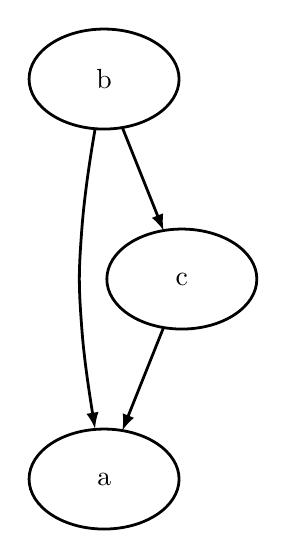
\begin{tikzpicture}[>=latex,line join=bevel,]
  \pgfsetlinewidth{1bp}
%%
\pgfsetcolor{black}
  % Edge: b -> a
  \draw [->] (23.752bp,143.89bp) .. controls (21.954bp,133.54bp) and (19.905bp,120.06bp)  .. (19.0bp,108.0bp) .. controls (17.803bp,92.045bp) and (17.803bp,87.955bp)  .. (19.0bp,72.0bp) .. controls (19.637bp,63.518bp) and (20.838bp,54.336bp)  .. (23.752bp,36.112bp);
  % Edge: c -> a
  \draw [->] (48.364bp,72.411bp) .. controls (45.087bp,64.216bp) and (41.056bp,54.14bp)  .. (33.588bp,35.47bp);
  % Edge: b -> c
  \draw [->] (33.636bp,144.41bp) .. controls (36.913bp,136.22bp) and (40.944bp,126.14bp)  .. (48.412bp,107.47bp);
  % Node: a
\begin{scope}
  \definecolor{strokecol}{rgb}{0.0,0.0,0.0};
  \pgfsetstrokecolor{strokecol}
  \draw (27.0bp,18.0bp) ellipse (27.0bp and 18.0bp);
  \draw (27.0bp,18.0bp) node {a};
\end{scope}
  % Node: c
\begin{scope}
  \definecolor{strokecol}{rgb}{0.0,0.0,0.0};
  \pgfsetstrokecolor{strokecol}
  \draw (55.0bp,90.0bp) ellipse (27.0bp and 18.0bp);
  \draw (55.0bp,90.0bp) node {c};
\end{scope}
  % Node: b
\begin{scope}
  \definecolor{strokecol}{rgb}{0.0,0.0,0.0};
  \pgfsetstrokecolor{strokecol}
  \draw (27.0bp,162.0bp) ellipse (27.0bp and 18.0bp);
  \draw (27.0bp,162.0bp) node {b};
\end{scope}
%
\end{tikzpicture}

